\begin{figure}
    \centering
    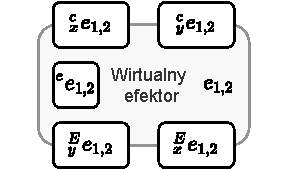
\includegraphics[width=0.75\columnwidth]{figures/ISR-ve-gripper-model.pdf}
    \label{fig:model-vr-camera}
    \caption{Struktura ogólna wirtualnego efektora chwytaka dwustanowego}
\end{figure}

\begin{figure}
    \centering
    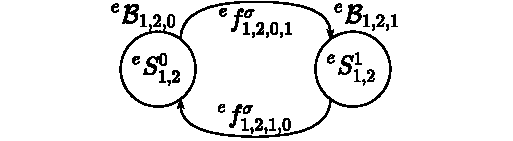
\includegraphics[width=\columnwidth]{figures/ISR-ve-gripper-behaviours.pdf}
    \label{fig:zachowania-ve-gripper}
    \caption{Automat zachowań wirtualnego efektora chwytaka dwustanowego}
\end{figure}

Zachowania:
\begin{itemize}
    \item ${}^{e}\mathcal{B}_{1,2,0}$ - open,
    \item ${}^{e}\mathcal{B}_{1,2,1}$ - close.
\end{itemize}

Bufory komunikacyjne:
\begin{itemize}
    \item ${}^{c}_{x}e_{1,2} = \xi^{\mathrm{cs}}_{\mathrm{zad}} \in \{o, c\}$ - zadany stan chwytaka,
    \item ${}^{c}_{y}e_{1,2} = \xi^{\mathrm{cs}} \in \{o, c\}$ - aktualny stan chwytaka,
    \item ${}^{E}_{x}e_{1,2} = \Xi \in \{o, c\}$ - aktualny stan chwytaka,
    \item ${}^{E}_{y}e_{1,2} = \Xi_{\mathrm{zad}} \in \{o, c\}$ - zadany stan chwytaka.
\end{itemize}

Warunki początkowe:
\begin{itemize}
    \item ${}^{e}f^{\sigma}_{1,2,0} \triangleq \xi_{\mathrm{zad}} = c$
    \item ${}^{e}f^{\sigma}_{1,2,1} \triangleq \xi_{\mathrm{zad}} = o$
\end{itemize}

Warunki końcowe:
\begin{itemize}
    \item ${}^{e}f^{\tau}_{1,2,0} \triangleq \xi_{\mathrm{zad}} \neq c$,
    \item ${}^{e}f^{\tau}_{1,2,1} \triangleq \xi_{\mathrm{zad}} \neq o$
\end{itemize}

Funkcje przejścia w postaci matematycznej:
\begin{itemize}
    \item \textbf{open} \begin{itemize}
        \item ${}^{e_{1,2}, E_{1,2}}f_{1,2,0} \triangleq {}^{E}_{y}e_{1,2} = o$,
        \item ${}^{e_{1,2}, c_{1,1}}f_{1,2,0} \triangleq {}^{c}_{y}e_{1,2} = o$,
    \end{itemize} 
    \item \textbf{close} \begin{itemize}
        \item ${}^{e_{1,2}, E_{1,2}}f_{1,2,1} \triangleq {}^{E}_{y}e_{1,2} = c$,
        \item ${}^{e_{1,2}, c_{1,1}}f_{1,2,1} \triangleq {}^{c}_{y}e_{1,2} = c$,
    \end{itemize}
\end{itemize}

\begin{figure}
    \centering
    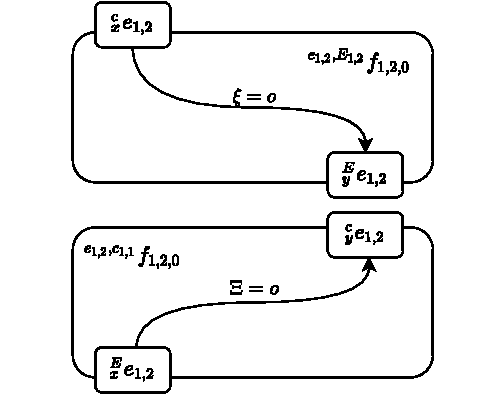
\includegraphics[width=\columnwidth]{figures/ISR-ve-gripper-fp-open.pdf}
    \label{fig:ve-gripper-fp-open}
    \caption{Zdekomponowana funkcja przejścia zachowania \textbf{open} w~postaci DFD}
\end{figure}

\begin{figure}
    \centering
    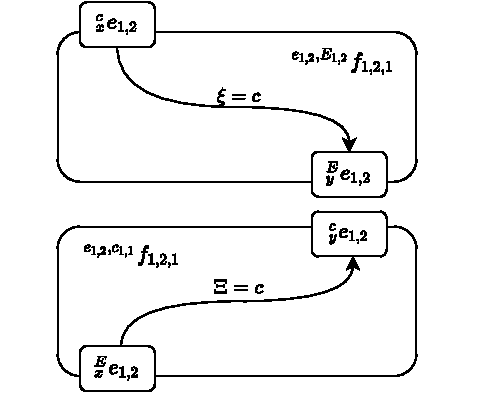
\includegraphics[width=\columnwidth]{figures/ISR-ve-gripper-fp-close.pdf}
    \label{fig:ve-gripper-fp-close}
    \caption{Zdekomponowana funkcja przejścia zachowania \textbf{close} w~postaci DFD}
\end{figure}